% -*-memoria.tex-*-
% Este fichero es parte de la plantilla LaTeX para
% la realización de Proyectos Final de Carrera, protejido
% bajo los términos de la licencia GFDL.
% Para más información, la licencia completa viene incluida en el
% fichero fdl-1.3.tex

% Copyright (C) 2009 Pablo Recio Quijano 

%-------------------------------------------------------
% ---- Plantilla para libros / memorias PFC -----

% Realizada por Pablo Recio Quijano y Noelia Sales Montes 
% Formato de portada y primera página tomado del PFC de
% Francisco Javier Vázquez Púa, en su proyecto 'libgann'
% -------------------------------------------------------

\documentclass[a4paper,11pt]{book}

\usepackage{./estilos/estiloBase} % Basicamente son todas las
                                  % librerias usadas. En caso de que
                                  % falten librerias se van añadiendo
                                  % al fichero.
\usepackage{./estilos/colores}  % Algunos colores ya generados, para
                                % los algunos estilos más avanzados.
\usepackage{./estilos/comandos} % Algunos comandos personalizados

\graphicspath{{./imagenes/}} % Indicamos la ruta donde se encuentran
                             % las imagenes, para ahorrarnos la ruta
                             % completa, y solo modificar aquí si en
                             % un momento dado lo movemos

\begin{document}

% Renombramos las figuras y las tablas
\renewcommand{\figurename}{Figura}
\renewcommand{\listfigurename}{Indice de figuras}
\renewcommand{\tablename}{Tabla}
\renewcommand{\listtablename}{Indice de tablas}


% PORTADA PABLO
\begin{titlepage}
 \begin{center}
  
  \vspace*{5cm}
  
  \textsc{\LARGE Universidad de Cádiz}\\[1.5cm]
  
  \textsc{\Large Administración de Sistemas Operativos}\\[0.5cm]
 
  
  % Title
  \HRule \\[0.4cm]
  { \huge \bfseries Sistemas para el Control de Versiones }\\[0.4cm]
  
  \HRule \\[1.5cm]
  
  % Author and supervisor
  \begin{minipage}{0.4\textwidth}
   \begin{flushleft} \large
    Rosa Mª Durante Lerate\\
    Pablo Recio Quijano
   \end{flushleft}
  \end{minipage}
  \begin{minipage}{0.4\textwidth}
   \begin{flushright} \large
    Leandro Pastrana González\\
    Noelia Sales Montes
   \end{flushright}
  \end{minipage}
  
  \vfill
  
 \end{center}
 
\end{titlepage}

\cleardoublepage


\frontmatter % Introducción, índices ...

%\input{previo.tex}
%\cleardoublepage

\tableofcontents
%\listoffigures
%\listoftables

\mainmatter % Contenido en si ...

\chapter[Introducción a los SS.C.VV.]{Introducción a los Sistemas de control de Versiones}
\section[¿Qué es un S.C.VV.?]{¿Qué es un Sistema de Control 
  de Versiones?}

Un Sistema de Control de Versiones (en adelante \textbf{SCV}), es un 
software que controla y organiza las distintas \textbf{revisiones} que 
se realizen sobre uno o varios documentos.

Pero, ¿qué es una revisión?. Se podría decir que una revisión es un cambio
realizado sobre un documento, por ejemplo añadir un parrafo, borrar un 
fragmento o algo similar. Veamos un ejemplo:\\

Supongamos que cargamos en un SCV el siguiente código fuente:

\begin{lstlisting}[style=C++]
#include <iostream>

int main(){
  cout << ''Hola, mundo!'' << endl;
}
\end{lstlisting}

Se añade al SCV como la revisión 1 del fichero. Una vez añadido, vemos que 
no compila, ya que nos falta incluir el uso del espacio de nombres, así
que lo modificamos:

\begin{lstlisting}[style=C++]
#include <iostream>

using namespace std;

int main(){
  cout << ''Hola, mundo!'' << endl;
}
\end{lstlisting}

Se vuelve a añadir al SCV, ahora como la revisión número 2. De esta forma, 
se guarda el \textbf{historial} de las distintas modificaciones sobre un 
fichero, por lo que en cualquier momento podemos restaurar la revisión que
queramos de un fichero.\\

Esto presenta varias ventajas, aunque la principal y la más llamativa es
que nos permite mantener una copia de seguridad de todas las modificaciones
realizadas sobre un fichero, lo cual nos facilita la tarea de deshacer algo
que esté mal. Supongamos por ejemplo que modificamos un proyecto software, y
modificamos un módulo para arreglar un bug.

Ahora funciona para ese bug, pero nos hemos ``cargado'' otra funcionalidad 
más importante, que no queremos perder. Simplemente volvemos a una revisión
anterior, y no hay problemas.

\section[¿Para qué sirve un S.C.VV.?]{¿Para qué sirve un Sistema de 
  Control de Versiones?}

De forma general, se utilizan SCV para desarrollo de proyectos Software, 
sobre todo para realizar en grupos de desarrollo. Vamos a analizar un poco
los motivos de porque esto es así.

\subsection{Ejemplo de grupo de desarrollo sin Sistema de Control de Versiones}

Supongamos un grupo de 5 desarrolladores, que están realizando un proyecto.
Puede ser que el proyecto esté muy claro que partes tiene que hacer cada uno,
pero esto no suele ser así.\\

Estos desarrolladores van subiendo a un servidor tipo FTP las distintas 
modificaciones que realizan sobre el código. Uno sube un fichero fuente 
\texttt{claseA.h}, otro \texttt{entrada-salida.cpp}, etc...

Sin embargo, llegará un momento en el que dos desarrolladores modifiquen
el mismo fichero. Veamos un ejemplo claro, con el siguiente código:

\begin{lstlisting}[style=C++]
#include <iostream>

using namespace std;

int main(){
  int *v = {1,2,3,5,9,10,3,2}; //esto no es correcto para el compilador, 
                               //pero nos vale conceputalmente.
  int a = 7 ,b = 3;

  // -------- Swap entre a y b
  int aux = a;
  a = b;
  b= aux;
  //--------------------------
  //------- Maximo de *v -----
  int max = v[0];
  for (int i = 0; i < 8 ; i++){
    if (v[i] > max){
      max = v[i];
    }
  }
  //--------------------------

  cout << ``a = `` << a << endl;
  cout << ``b = `` << b << endl;
  cout << ``max de v = `` << max << endl;
}
\end{lstlisting}

Ahora, el desarrollador Pepe decide modular algo más el código, y añadir
una función que realize el swap de dos variables enteras, quedando el siguiente
código:

\begin{lstlisting}[style=C++]
#include <iostream>

using namespace std;

void swap(int &a, int &b);

int main(){
  int *v = {1,2,3,5,9,10,3,2}; //esto no es correcto para el compilador, 
                               //pero nos vale conceputalmente.
  int a = 7 ,b = 3;

  // -------- Swap entre a y b
  swap(a,b);
  //--------------------------
  //------- Maximo de *v -----
  int max = v[0];
  for (int i = 0; i < 8 ; i++){
    if (v[i] > max){
      max = v[i];
    }
  }
  //--------------------------

  cout << ``a = `` << a << endl;
  cout << ``b = `` << b << endl;
  cout << ``max de v = `` << max << endl;
}

void swap(int &a, int &b){
  int aux = a;
  a = b;
  b= aux;
}
\end{lstlisting}

Realiza el cambio y sube el fichero al servidor FTP, ``machacando'' el que
ya estaba ahí. Ahora resulta que en el intervalo de tiempo en el que el
desarrollador Pepe estaba realizando la función \texttt{swap()}, la
desarrolladora \texttt{María}, decide realizar una función que localize el
máximo de un vector y lo devuelva, ya que considera que se puede utilizar en
muchos más sitios:

\begin{lstlisting}[style=C++]
#include <iostream>

using namespace std;

int maximo(int *v, int tam);

int main(){
  int *v = {1,2,3,5,9,10,3,2}; //esto no es correcto para el compilador, 
                               //pero nos vale conceputalmente.
  int a = 7 ,b = 3;

  // -------- Swap entre a y b
  int aux = a;
  a = b;
  b= aux;
  //--------------------------
  //------- Maximo de *v -----
  int max = maximo(v,8);
  //--------------------------

  cout << ``a = `` << a << endl;
  cout << ``b = `` << b << endl;
  cout << ``max de v = `` << max << endl;
}

int maximo(int *v, int tam){
  int max = v[0];
  for (int i = 0 ; i < tam ; i++){
    if (v[i] > max){
      max = v[i];
    }
  }
}
\end{lstlisting}

Ella, descargó la revisión anterior a la modificación de Pepe, por lo que sube
el fichero, y ``machaca'' la versión anterior, que es la que habia hecho Pepe,
eliminando su trabajo, el cual además era complementario al de María. Por tanto
la próximo vez que Pepe compruebe el servidor, verá que lo que hizo ya no está.\\

Aquí entran en juego los sistemas de control de versiones. Si el grupo de desarrollo
usara un SCV, esto no pasaría, ya que estos sistemas vigilan sobre que lineas se han
hecho estas modificaciones, de forma que ``verían'' que los dos cambios no son
incompatibles, y en la nueva versión, \textit{mergerá} las dos modificaciones.

Incluso sin esta función, el problema de conflicto, sería más facilmente resoluble,
ya que al mantener versiones anteriores se pueden rescatar, para ver que cambios se
han hecho y realizar esa unión de forma manual, aunque si es automatizable, mejor.\\

Extrapolemos esto a cualquier desarrollo de software con un grupo relativamente grande, como
por ejemplo los desarrolladores de cualquier proyecto de Software Libre medianamente grande, 
en el cual puede haber decenas de personas distintas implicadas en el desarrollo. Si fuera
un grupo como el descrito arriba, el desarrollo puede llegar a ser un auténtico caos. Por este
motivo se hace indispensable el uso de alguna herramientas de SCV en desarrollos de software
mayores que los unipersonales.

Aunque no está restringido solo al software, ya que trabaja con cualquier tipo de ficheros de texto
plano, por lo que también se puede usar para generar documentación de forma colaborativa usando
\LaTeX{} por ejemplo \footnote{Los profesores del departamento de Estadística, lo usan para el
libro de R}

\subsection{Ejemplos en el Software Libre}

Hemos visto antes que fundamentalmente el uso de SCV está destinado al desarrollo de Software,
ayudando a la sincronización de los distintos miembros del grupo de desarrollo. Esto se cumple tanto
en entornos privados (empresas) como en entornos públicos (proyectos libres). Veamos algunos ejemplos
de proyectos libres que utilizan estas herramientas:

\begin{description}
\item[Kernel de Linux: ] Utiliza \textbf{Git} desde el año 2005. Previamente 
  utilizaba \textbf{BitKeeper}
\item[KDE: ] Utiliza \textbf{Subverion}. A fecha del 2 de Mayo de 2009, andan por la revisión 
  962574, cerca de un millón, habiendo sido la primera en el año 1997. Actualmente trabajan en
  el proyecto más de 200 personas. ¿Imaginamos como sería sincronizar todas estas personas sin
  un SCV? Es totalmente imposible.
\item[Firefox: ] Utilizan \textbf{CVS}.
\item[Ubuntu: ] Utiliza \textbf{Bazaar}, un sistema distribuido.
\end{description}

Podríamos continuar la lista con muchísimos más. Por ejemplo, los sistemas de forjas 
(\texttt{sourceforge.net}, \texttt{forja.rediris.es}, etc...) dan soporte para SCV, incluyendo
herramientas para navegar en el arbol del repositorio.

\section{Tipos de Sistemas de Control de Versiones}

Fundamentalmente, podemos distinguir dos tipos distintos de SCV: \textbf{centralizados} y 
\textbf{distribuidos}.

\subsection{Sistemas centralizados}

Presentan la característica fundamental de que funcionan como un entorno clásico \textit{Cliente-
  Servidor}. Es decir, tendremos un servidor en el que se alojará el respositorio del proyecto,
con toda la información de los cambios, ficheros binarios añadidos, etc...

En estos sistemas, el cliente trabaja con una ``copia de trabajo'' del servidor, la cual es 
realmente una copia de como estaba el servidor en una revisión determinada, normalmente es la más
actualizada. El desarrollador hace cambios sobre esa copia de trabajo, y cuando considera que ha
terminado con esa modificación la sube (\textbf{commit}) al servidor, el cual se encargará de 
fundir esos cambios en el respositorio central, resolver conflictos si pudiera, ó informar al usuario
de los errores que se hayan podido dar.

Además, estos sistemas pueden a su vez dividirse en dos tipos más, según la forma que tengan de
controlar los posibles conflictos sobre un mismo fichero desde más de un cliente:

\subsubsection{Bloqueo del archivo}

Aplicando el principio de exclusión mutua, estos sistemas lo que hace es muy simple: cuando alguien
está modificando un archivo, bloquea el acceso de escritura a ese archivo para el resto de usuarios.

Esto implica que habrá menos conflictos cuando se fundan distintas ramas, pero presentan una enorme
cantidad de problemas extra:

\begin{itemize}
\item Alguien puede ``olvidarse'' de abrir el archivo para el resto.
\item Puede ocasionar que alguien trabaje de forma local para evitar el cerrojo, 
  y a la hora de fundir los cambios sea aun peor.
\end{itemize}

\subsubsection{Fusión de versiones}

Es el usado en la mayoria de los SCV. Es lo que se explicó en el ejemplo anterior: el SCV controla
que lineas del código se han cambiado en cada revisión, por lo que si dos desarrolladores cambian
zonas distintas de un mismo fichero, el sistema podrá fundir ambos cambios en la versión
del servidor.\\

Sin embargo, estos sistemas pueden fallar por un simple indentado, una linea de más o de menos, 
y en muchas ocasiones es el programador quien debe corregir esos conflictos a mano, que en muchos
casos es bastante problemático.

\subsection{Sistemas distribuidos}

Si los sistemas centralizado utiliza un modelo clásico de entorno \textit{cliente-servidor}, se
podría decir que un sistema distribuido es similar a un sistema \textit{Peer-to-Peer (P2P)}.

En estos sistemas, en lugar de que cada cliente tiene una copia de trabajo del (único) servidor,
la copia de trabajo de cada cliente es un respositorio en si mismo, una rama nueva del proyecto
central. De esta forma, la sincronización de las distintas ramas se realiza intercambiando 
``parches'' con otros clientes del proyecto. Esto es claramente un enfoque \textbf{muy} 
diferente al de los sistemas centralizados, por diversos motivos:

\begin{itemize}
\item No hay una copia original del código del proyecto, solo existen las distintas copias 
  de trabajo.
\item Operaciones como los commits, mirar el historial o rehacer cambios, no necesitan de una
  conexión con un servidor central, esta conexión solo es necesaria al ``compartir'' tu rama con
  otro cliente del sistema.
\item Cada copia de trabajo es una copia remota del código fuente y de la historia de cambios, 
  dando una seguridad muy natural contra la pérdida de los datos.
\end{itemize}


\chapter{Funcionamiento para el cliente}


\section{Introducción al cliente en un \textbf{SCV}}

Todos los sistemas de control de versiones se basan en disponer de un  
\textbf{repositorio}, que es el conjunto de información gestionada por
el sistema. Este repositorio contiene el historial de versiones de
todos los elementos gestionados. Con lo cual, lo primero que debe
hacer el cliente es obtener su copia de trabajo del repositorio;
dependiendo de que tipo de \textbf{Sistema de Control de Versiones}
utilice se obtendrá la copia de trabajo de una forma u otra.\\

A partir de este momento ya el cliente podrá realizar sus aportes al
repositorio. Para ello, el cliente trabajara bajo su copia de trabajo
y realizará las modificaciones oportunas. Sin embargo, esas
modificaciones no se tendrán en cuenta en el repositorio hasta que no
se envíen al él. \\

Aunque los tipos de \textbf{SCV} son muy distintos entre ellos, desde
el punto de vista del cliente no lo son tanto: el hecho de que el
repositorio se organice de forma distribuida o centralizada no afecta
al estilo de trabajo del cliente. \\

\subsection{Términos básicos}
\begin{description}
\item [Repositorio] Es el lugar donde se almacenan los datos
  actualizados e históricos en un servidor.
\item [Módulo] Conjunto de directorios y/o archivos dentro del
  repositorio que pertenecen a un proyecto común. 
\item [Rotular (tag)] Darle a alguna versión de cada uno de los
  ficheros del módulo en desarrollo en un momento preciso un nombre
  común ("etiqueta" o "rótulo") para asegurarse de reencontrar ese
  estado de desarrollo posteriormente bajo ese nombre. 
\item [Versión] Una revisión es una versión determinada de un
  archivo. 
\item [Ramificar (branch)] Un módulo puede ser bifurcado en un momento
  de tiempo de forma que, desde ese momento en adelante, dos copias de
  esos ficheros puedan ser desarrolladas a diferentes velocidades o de
  diferentes formas, de modo independiente. 
\item [Desplegar (check-out)] Un despliegue crea una copia de trabajo
  local desde el repositorio. Se puede especificar una revisión
  concreta, y por defecto se suele obtener la última. 
\item [Envío (commit)] Una copia de los cambios hechos a una copia
  local es escrita o integrada sobre repositorio. 
\item [Conflicto] Puede ocurrir en varias circunstancias:
\begin{itemize}
\item Los usuarios X e Y despliegan versiones del archivo A en que las
  líneas n1 hasta n2 son comunes. 
\item El usuario X envía cambios entre las líneas n1 y n2 al archivo A.
\item El usuario Y no actualiza el archivo A tras el envío del usuario X.
\item El usuario Y realiza cambios entre las líneas n1 y n2.
\item El usuario Y intenta posteriormente enviar esos cambios al archivo A.
\end{itemize}
En estos casos el sistema es incapaz de fusionar los cambios y pide al
usuario que sea él quien \textbf{resuelva} el conflicto. 
\item [Resolver] El acto de la intervención del usuario para atender
  un conflicto entre diferentes cambios al mismo documento. 
\item [Cambio (diff)] Un cambio representa una modificación específica
  a un documento bajo control de versiones. 
\item [Lista de Cambios (changelist)] En muchos sistemas de control de
  versiones con commits multi-cambio atómicos, una lista de cambios
  identifica el conjunto de cambios hechos en un único commit. 
\item [Exportación] Una exportación es similar a un check-out, salvo
  porque crea un árbol de directorios limpio sin los metadatos de
  control de versiones presentes en la copia de trabajo. 
\item [Importación] Una importación es la acción de copia un árbol de
  directorios local (que no es en ese momento una copia de trabajo) en
  el repositorio por primera vez.
\item [Fusión (merge)] Una integración o fusión une dos conjuntos de
  cambios sobre un fichero o un conjunto de ficheros en una revisión
  unificada de dicho fichero o ficheros. Puede suceder cuando: 
\begin{itemize}
\item Un usuario, trabajando en esos ficheros, actualiza su copia
  local con los cambios realizados, y añadidos al repositorio, por
  otros usuarios. Análogamente, este mismo proceso puede ocurrir en el
  repositorio cuando un usuario intenta check-in sus cambios. 
\item Después de que el código haya sido branched, y un problema
  anterior al branching sea arreglado en una rama, y se necesite
  incorporar dicho arreglo en la otra. 
\item Después de que los ficheros hayan sido branched, desarrollados
  de forma independiente por un tiempo, y que entonces se haya
  requerido que fueran fundidos de nuevo en un único trunk unificado. 
\end{itemize}
\item [Integración inversa] El proceso de fundir ramas de diferentes
  equipos en el trunk principal del sistema de versiones. 
\item [Actualización (update)] Una actualización integra los cambios
  que han sido hechos en el repositorio (por ejemplo por otras
  personas) en la copia de trabajo local. 
\item [Copia de trabajo] La copia de trabajo es la copia local de los
  ficheros de un repositorio, en un momento del tiempo o revisión
  específicos. Todo el trabajo realizado sobre los ficheros en un
  repositorio se realiza inicialmente sobre una copia de trabajo, de
  ahí su nombre. Conceptualmente, es un cajón de arena o sandbox. 
\item [Congelar] congelar significa permitir los últimos cambios
  (commits) para solucionar las fallas a resolver en una entrega
  (release) y suspender cualquier otro cambio antes de una entrega,
  con el fin de obtener una versión consistente. 
\end{description}

\section{Ciclo de trabajo con \textbf{SCV} centralizado: Subversion}

Cuando un cliente quiere comenzar a desarrollar un proyecto utilizando
Subversion primeramente debe instalar la herramienta de la siguiente
forma: 
\begin{lstlisting}[style=consola]
sudo apt-get install subversion
\end{lstlisting}

Cuando ya tiene la herramienta lista para utilizar ejecutará el
\textit{checkout} inicial:  
\begin{lstlisting}[style=consola]
svn checkout http://ruta/repositorio 
\end{lstlisting}
Por ejemplo: 
\begin{lstlisting}[style=consola]
svn checkout http://192.168.2.101/svn/RepositorioEjemplo 
\end{lstlisting}

A partir de este momento el cliente ya tiene en su poder una copia de
trabajo del repositorio en el cual podrá ejercer sus modificaciones e
incluirlas en el sistema de control de versiones. El ciclo de trabajo
que se debe llevar es el siguiente: 

\begin{itemize}
\item Actualizar la copia de trabajo (por si otros compañeros han
  realizado modificaciones):  
\begin{lstlisting}[style=consola]
svn update
\end{lstlisting}

\item Examinar los cambios a partir de comentarios en las
  revisiones. Cada vez que se envían las modificaciones al servidor se
  incluye un comentario sobre qué es lo que se ha modificado para esa
  revisión. Estos comentarios son los \textit{logs}. Para ver los logs
  se introduce en consola la siguiente línea de comandos: 
\begin{lstlisting}[style=consola]
svn log -r revmenor:revmayor 
\end{lstlisting}

De esta forma se mostrará en pantalla los comentarios de cada revisión
para informarnos de las modificaciones que se han realizado en
ellas. Esto es muy útil ejecutarlo antes de ponernos a modificar para
informarnos de cómo va el proyecto. 

\item Realizar los cambios pertinentes a los ficheros y directorios:
  mover, copiar, borrar, crear... (por ahora serán cambios
  locales). Hay que hacerlos con la asistencia de \textbf{svn}. De
  esta forma se mantendrá el historial de cambios. Se utiliza de la
  siguiente forma: 
\begin{lstlisting}[style=consola]
svn add [fichero|directorio]
svn mkdir directorio
svn delete [fichero|directorio]
svn mv [fichero|directorio]Original [fichero|directorio]Cambiado
svn cp [fichero|directorio]Original [fichero|directorio]Copiado
\end{lstlisting}

Veamos varios ejemplos de uso de estos comandos:
\begin{lstlisting}[style=consola]
svn add fichero1.c                         // creamos fichero1.c
svn add fichero2.c                         // creamos fichero2.c
svn mkdir dirficheritos                    // creamos dirficheritos
svn cp fichero1.c ficheritos/fichero1.h    // copiamos el fichero
svn mv fichero2.c ficheritos/fichero1.cpp  // movemos el fichero
svn delete fichero1.c                      // borramos fichero1.c
\end{lstlisting}

\item Examinar los cambios realizados. Podemos comprobar el estado de
  los ficheros de la copia de trabajo de la siguiente forma: 
\begin{lstlisting}[style=consola]
svn status
\end{lstlisting}

Este comando muestra todos los cambios realizados en la copia de
trabajo desde que se realizó el último \textbf{svn update}. Puede
funcionar sin red ya que sólo es necesario tener las carpetas ocultas
\textit{.svn}. Los códigos más comunes que nos muestra son: 
\begin{itemize}
\item \textbf{A} fichero o directorio añadido.
\item \textbf{D} fichero o directorio borrado.
\item \textbf{U} fichero o directorio actualizado con cambios
  remotos. 
\item \textbf{M} fichero o directorio modificado localmente.
\item \textbf{G} fichero o directorio acutalizado con cambios locales
  y remotos reunidos automáticamente. 
\item \textbf{C} los cambios locales y remotos han de ser reunidos
  localmente (conflicto en modificaciones). 
\item \textbf{?} fichero o directorio que no se haya bajo el sistema
  de control de versiones y no se está ignorando. 
\item \textbf{!} fichero o directorio falta en el sistema de control
  de versiones (puede haberse borrado localmente). 
\item \textbf{~} el fichero o directorio no es del tipo esperado (se
  obtiene un directorio y se esperaba un fichero o viseversa) .
\item \textbf{+} se copiará información de historial además de
  contenido. 
\end{itemize}

\item Examinar las diferencias de ficheros entre dos revisiones. Ésto
  es útil cuando queremos enviar modificaciones cuando no tenemos
  acceso de escritura o para ver que han modificado los
  compañeros. Por defecto compara la revisión modificada localmente
  con la última registrada en el servidor. El comando a utilizar es: 
\begin{lstlisting}[style=consola]
svn diff [-r revmenor:revmayor] fichero
\end{lstlisting}

\item Deshacer posibles cambios en un fichero o directorio:
\begin{lstlisting}[style=consola]
svn revert fichero
\end{lstlisting}
Esto restaura al fichero obtenido al del último \textit{svn update}.

\item Resolver conflictos. Es muy conveniente el realizar un
  \textit{svn update} antes de subir nuestras modificaciones por si
  existiesen conflictos. 

\item Por último, para poder enviar las modificaciones al servidor
  usaremos el comando:
  \begin{lstlisting}[style=consola]
    svn commit -m log\_entre\_comillas
  \end{lstlisting}
  De esta forma quedarán almacenadas en el servidor las modificaciones
  realizadas en nuestra copia de trabajo además de la pequeña
  descripción que aportamos sobre éstas.
\end{itemize}
  

\section{Ciclo de trabajo con \textbf{SCV} distribuido: Git}

Como en todos los sistemas de control de versiones tenemos que
instalar la aplicación. Para \textit{Git} esto se hace con el
siguiente comando:
\begin{lstlisting}[style=consola]
  sudo apt-get install git-core
\end{lstlisting}

Para comenzar con \textit{Git} primero tenemos que introducir nuestros
datos (nombre y correo electrónico) para que el sistema nos indique
como autor en cada una de nuestras revisiones. Además podemos informar
a \textit{Git} de cuál es nuestro editor favorito (por defecto usa
Vim). Realizamos:
\begin{lstlisting}[style=consola]
  git config --global user.name ``Nombre Apellidos''
  git config --global user.email micorreo@ejemplo.com
  git config --global user.editor mieditor
\end{lstlisting}

Para comenzar con el ciclo de trabajo tenemos que crear nuestro
repositorio vacío, o clonar uno existente. También tenemos que tener
en cuenta si podrá acceder al repositorio varios usuarios. Crearemos
un directorio vacío para, a partir de él crear un repositorio vacío
y que se pueda compartir con todos los miembros del grupo al que
pertenezcan los ficheros del repositorio.
\begin{lstlisting}[style=consola]
  mkdir directorioVacio
  git init --shared=group
\end{lstlisting}

Podemos observar que se ha creado un directorio oculto
\textit{.git}. Contiene:
\begin{itemize}
  \item \textbf{config} Fichero con la configuración local de Git para
    este repositorio.
  \item \textbf{description} Descripción del repositorio para
    \textit{gitweb}
  \item \textbf{HEAD} Referencia a la revisión actual con la que
    trabajamos.
  \item \textbf{hooks} Guiones bash o programas para responder ante
    eventos.
  \item \textbf{info/exclude} Fichero del estilo de
    \textit{.gitignore} global para el repositorio y no controlado
    por Git.
  \item \textbf{object} Base de datos de objetos.
  \item \textbf{refs} Referencias por nombre a las puntas de las
    distintas ramas locales y remotas y a otras revisiones etiquetadas
    por nombre. 
\end{itemize}

Para saber el estado de los ficheros en \textit{Git} tenemos el
comando:
\begin{lstlisting}[style=consola]
  git status
\end{lstlisting}

Si en el directorio anterior creamos un fichero f cualquiera y
ejecutamos el comando anterior obtenemos la siguiente salida:
\begin{lstlisting}[style=consola]
  # On branch master
  #
  # Initial commit
  #
  # Untracked files:
  # (use "git add <file>..." to include in what will be committed)
  #
  # f
  nothing added to commit but untracked files present (use "git add" to track)
\end{lstlisting}

Con esto sabemos que:
\begin{itemize}
  \item Nos encontramos en la rama principal del repositorio creado.
  \item La siguiente revisión que creamos será la primera.
  \item Existen algunos fichero cuyos cambios no están monitorizados
    (añadidos al repositorio). En nuestro caso, nos está avisando que
    faltaría añadir el fichero f.
\end{itemize}

Veamos pues cómo podemos añadir ficheros para prepararlos para envío.
\begin{lstlisting}[style=consola]
  git add f
\end{lstlisting}

También podemos borrar ficheros con la siguiente orden:
\begin{lstlisting}[style=consola]
  git rm fichero
\end{lstlisting}

Ahora enviaremos las modificaciones y crearemos la primera revisión
con:
\begin{lstlisting}[style=consola]
  git commit -m comentario\_de\_la\_revision
\end{lstlisting}

Hay que tener en cuenta que con \textit{Git} trabajamos con tres
estructuras de datos: el repositorio (el directorio .git), el índice o
caché (.git/index) y la copia de trabajo (todo lo que está fuera de .git).

Con lo cual podemos comparar qué estados tiene cada directorio y qué
diferencias existen con la siguiente orden:
\begin{lstlisting}[style=consola]
  git diff
\end{lstlisting}

Obteniendo las diferencias entre el directorio de trabajo y la versión
preparada para envío en el índice, además de destacar aquella línea
que no preparemos para envío.

\begin{lstlisting}[style=consola]
  git diff --cached
\end{lstlisting}

Esta orde compara la versión del índice con la versión de la revisión
actual (HEAD), y así nos señalará que versión tenemos preparada para
enviar.

Para poder deshacer cambios en \textit{Git} podemos restaurar un
fichero del directorio de trabajo a la versión que se halle en el
índice de la siguiente forma:
\begin{lstlisting}[style=consola]
  git checkout fichero
\end{lstlisting}

Las formas más comunes de deshacer cambios en un fichero son: \\
\begin{tabular}{c c c}
\hline
Acción a deshacer & Afecta a & Orden \\
\hline
Añadido & & \\ 
Modificado & índice & git reset -- f \\
Borrado & & \\
\hline
Añadido & &  rm f \\
Modificado & dir.trabajo & git checkout f \\
Borrado & & git checkout f \\
\hline
Añadido & & git rm -f f \\
Modificado & ambos & git checkout HEAD f \\
Borrado & & git checkout HEAD f \\
\hline
\end{tabular}

Si no hemos enviado aún nuestros cambios a ningún otro repositorio ni
nadie nos ha tomado de nuestro repositorio podemos corregir errores
fácilmente en la última revisión que hayamos hecho:

\begin{lstlisting}[style=consola]
  git commit --amend
\end{lstlisting}

Con esto la anterior revisión se ignorará y será efectivamente
sustituida por otra que incorporará sus cambios y los que hayamos
hecho ahora.

Para poder etiquetar una revisión ejecutamos:
\begin{lstlisting}[style=consola]
  git tag etiqueta
\end{lstlisting}

También podemos etiquetar cualquier otra revisión creando objetos
reales de tipo ``etiqueta'' con comentarios (-a) y firmada con nuestra
clave pública GnuPG (-s) que tenga el mismo correo y nombre que le
dimos a \textit{Git}:

\begin{lstlisting}[style=consola]
  git tag -a -s etiqueta revision
\end{lstlisting}

Finalmente podemos redistribuir los contenidos de cualquier revisión
mediante la orden :

\begin{lstlisting}[style=consola]
  git archive etiqueta\_de\_la\_revision
\end{lstlisting}




\chapter{El servidor en Sistemas Centralizados}
% Sistemas de control de versiones centralizados


 \section{Introducción}
 
  \subsection{Los paradigmas en Sistemas de Control de Versiones}
  
  Desde hace tiempo, la tendencia de uso de los sistemas de control de
  versiones, ha sido el uso centralizado mediante sistemas tan populares
  como CVS o Subversion. Ahora, desde que muchos grandes proyectos
  optaran por los sistemas de control de versiones distribuidos, cada
  vez hay más gente que se va cambiando a ellos y, sobre todo, proyectos
  grandes.

  ¿Será que es mejor el enfoque distribuido al centralizado?
  
  \subsection{Sistemas centralizados}
  
  En un sistema de control de versiones centralizado todos nuestros
  fuentes y sus versiones están almacenados en un único directorio
  (llamado repositorio de fuentes) de un ordenador (un servidor). Todos
  los desarrolladores que quieran trabajar con esos fuentes, deben
  pedirle al sistema de control de versiones una copia local para
  trabajar. En ella realizan todos sus cambios y cuando están listos y
  funcionando, le dicen al sistema de control de versiones que guarde
  los fuentes modificados como una nueva versión.
  
  Es decir, funcionan según el paradigma clásico cliente-servidor.
  
  Una vez subido el código, está disponible para otros desarrolladores,
  que pueden actualizarse y pedir la nueva versión. De alguna forma,
  para el intercambio de fuentes entre ellos, es necesario pasar por el
  repositorio de fuentes del servidor. Es en el servidor donde están
  guardadas todas las versiones y los desarrolladores sólo tienen en su
  copia local aquellos fuentes que han solicitado del servidor.

  Los sistemas de control de versiones gratuitos más conocidos son CVS y
  Subversion. 
  
 \section{El enfoque Centralizado}
 
 Cuando se desarrollaron los sistemas de control de versiones, muchos de
 ellos se hicieron en esquema cliente-servidor, con lo que el desarrollo
 de las herramientas está claramente diferenciado entre:
 
 \begin{itemize}
  \item el cliente, que es la aplicación que se conecta al servidor y
	mantiene una copia local del repositorio, así como se encarga,
	generalmente de la corrección de conflictos y la mayoría de
	lógica del sistema.
  \item el servidor, que es el sistema que toma los datos del cliente y
	los almacena a espera de una o múltiples peticiones de esos
	datos. Este sistema se encargaría del almacenamiento de las
	versiones, control de concurrencia, bloqueos y otras
	características parecidas a las de las bases de datos.
 \end{itemize}
 
 ¿Qué limitaciones y características posee? Haremos una breve lista:
 
 \begin{itemize}
  \item El sistema servidor es un repositorio, como los que mantienen
	los clientes, pero perfectamente sincronizado y sin que dé lugar
	a conflictos. Es la copia maestra de los datos.
  \item Cuando un sistema web quiere hacer un listado, puede tomar los
	datos de este servidor y siempre serán seguros, con lo que no
	tendrá que resolver conflictos, ni tendrá que hacer mezclas.
  \item Una copia local debe de poder mezclarse con el repositorio
	central cuando queramos publicar un conjunto de cambios o cuando
	queramos tomar la última versión publicada en concordancia con
	nuestra copia local.
  \item Es normal ver en muchos de estos sistemas ramificaciones,
	versiones, etiquetas, o similares, a modo de tener varias copias
	según nos interese. Estas ramificaciones están en el servidor y
	en algunos casos puede llegar a ser muy costosa su
	diferenciación.
 \end{itemize}
 
 
 
 \section{CVS}
 
  \subsection{Introducción}
  
  El Concurrent Versions System (CVS), también conocido como Concurrent
  Versioning System, es una aplicación informática que implementa un
  sistema de control de versiones: mantiene el registro de todo el
  trabajo y los cambios en los ficheros (código fuente principalmente)
  que forman un proyecto (de programa) y permite que distintos
  desarrolladores (potencialmente situados a gran distancia)
  colaboren. CVS se ha hecho popular en el mundo del software libre. Sus
  desarrolladores difunden el sistema bajo la licencia GPL.
  
  \subsection{Características}
  
  CVS utiliza una arquitectura cliente-servidor: un servidor guarda
  la(s) versión(es) actual(es) del proyecto y su historial. Los clientes
  se conectan al servidor para sacar una copia completa del
  proyecto. Esto se hace para que eventualmente puedan trabajar con esa
  copia y más tarde ingresar sus cambios con comandos GNU.
  
  Típicamente, cliente y servidor se conectan utilizando Internet, pero
  con el sistema CVS el cliente y servidor pueden estar en la misma
  máquina. El sistema CVS tiene la tarea de mantener el registro de la
  historia de las versiones del programa de un proyecto solamente con
  desarrolladores locales. Originalmente, el servidor utilizaba un
  sistema operativo similar a Unix, aunque en la actualidad existen
  versiones de CVS en otros sistemas operativos, incluido Windows. Los
  clientes CVS pueden funcionar en cualquiera de los sistemas operativos
  más difundidos.
  
  Varios clientes pueden sacar copias del proyecto al mismo
  tiempo. Posteriormente, cuando actualizan sus modificaciones, el
  servidor trata de acoplar las diferentes versiones. Si esto falla, por
  ejemplo debido a que dos clientes tratan de cambiar la misma línea en
  un archivo en particular, entonces el servidor deniega la segunda
  actualización e informa al cliente sobre el conflicto, que el usuario
  deberá resolver manualmente. Si la operación de ingreso tiene éxito,
  entonces los números de versión de todos los archivos implicados se
  incrementan automáticamente, y el servidor CVS almacena información
  sobre la actualización, que incluye una descripción suministrada por
  el usuario, la fecha y el nombre del autor y sus archivos log.
  
  Los clientes pueden también comparar diferentes versiones de archivos,
  solicitar una historia completa de los cambios, o sacar una "foto"
  histórica del proyecto tal como se encontraba en una fecha determinada
  o en un número de revisión determinado. Muchos proyectos de código
  abierto permiten el "acceso de lectura anónimo", significando que los
  clientes pueden sacar y comparar versiones sin necesidad de teclear
  una contraseña; solamente el ingreso de cambios requiere una
  contraseña en estos casos.

  Los clientes también pueden utilizar la orden de actualización con el
  fin de tener sus copias al día con la última versión que se encuentra
  en el servidor. Esto elimina la necesidad de repetir las descargas del
  proyecto completo.
  
  CVS también puede mantener distintas "ramas" de un proyecto. Por
  ejemplo, una versión difundida de un proyecto de programa puede formar
  una rama y ser utilizada para corregir errores. Todo esto se puede
  llevar a cabo mientras la versión que se encuentra actualmente en
  desarrollo y posee cambios mayores con nuevas características se
  encuentre en otra línea formando otra rama separada.
  
  \subsection{Estado actual}
  
  VS fue desarrollado por GNU, el sitio GNU distribuye el programa,
  denominándolo "paquete GNU" con aplicaciones básicas a través de esta
  página. En otros proyectos se otorga con licencia GPL.
  
  Actualmente existen muchas versiones de CVS implantadas en los
  diferentes sistemas operativos.
  
  
  \subsection{Limitaciones del protocolo CVS}
  
  Los archivos en el repositorio sobre la plataforma CVS no pueden ser
  renombrados, estos deben ser agregados con otro nombre y luego
  eliminados. El protocolo CVS no provee una manera de que los
  directorios puedan ser eliminados o renombrados, cada archivo en cada
  subdirectorio debe ser eliminado y re-agregado con el nuevo
  nombre. Soporte limitado para archivos Unicode con nombres de archivo
  no ASCII.

  
  \subsection{Requisitos mínimos}
  
  CVS requiere dos programas.
  
  Por un lado un servidor instalado en un ordenador. Este servidor es el
  que guardará todas las versiones de todos nuestros ficheros. Es al que
  le mandaremos nuestros ficheros cuando los tengamos listos y el que
  nos devolverá dichos ficheros cuando se los pidamos.
  
  Por otro lado, en nuestro ordenador de trabajo necesitamos un cliente
  de CVS. Este es un programa capaz de conectarse con el servidor y
  pedirle o enviarle ficheros fuentes, según nosotros lo vayamos
  necesitando. Para windows hay un programa cvs.exe que se ejecuta desde
  la línea de comandos de ms-dos. Será ese el que usemos, ya que nos
  permitirá aprender los comandos típicos de CVS. 
  

  \subsection{Utilización y comandos}
  
  Suponemos instalado un servidor de CVS en algún ordenador. Vamos a ver
  las cosas que podemos hacer en el orden en que habitualmente se hacen.
  
  %cvs import ---> Creación de un proyecto
  
  Alguien, en su ordenador crea toda la estructura de directorios para
  un proyecto. Pone directorios para los fuentes, ficheros de
  configuración, scripts de compilado, imágenes, algo de código fuente,
  etc, etc.
  
  Para guardar esa primera versión del proyecto primero debemos declarar
  la variable de entorno CVSROOT de la siguiente forma.
  
  %C:\> set CVSROOT=:pserver:usuario@servidor:directorio
  
  donde:
  
  \begin{itemize}
   \item usuario es el nombre del usuario que va crear el proyecto. El
	 nombre de usuario debe ser conocido por el servidor de CVS.
   \item servidor es el nombre del ordenador en el que corre el servidor
	 de CVS.
   \item directorio es el directorio en el ordenador del servidor donde
	 se almacenan nuestros fuentes. 
  \end{itemize}
  
  Por supuesto, estas tres cosas deben ser conocidas y estar
  configuradas en el servidor de CVS.
  
  Una vez definida la variable, hay que entrar en sesión
  
  %C:\> cvs login
  %password:
  
  El comando cvs login sólo es necesario ejecutarlo una vez en la
  vida. La sesión permanecerá abierta incluso aunque apaguemos el
  ordenador. La única forma de salir de la sesión es ejecutando cvs
  logout
  
  Ejecutando cvs login nos pedirá la password para el usuario. Debe ser
  por supuesto la que tengamos para el servidor de CVS.
  
  Ahora nos vamos al directorio donde esté nuestro proyecto y ejecutamos
  el comando
  
  %C:\> cvs import PROYECTO etiqueta1 etiqueta2
  
  donde:
  
  \begin{itemize}
   \item PROYECTO es el nombre que queramos dar a nuestro proyecto. No
	 puede haber en CVS dos proyectos con el mismo nombre.
   \item etiqueta1 es una etiqueta cualquiera. Habitualmente se suele
	 poner el nombre de la empresa.
   \item etiqueta2 es otra etiqueta cualquiera. Suele ponerse algo
	 relativo a la versión. 
  \end{itemize}
  
  
  Este comando llevará a CVS todos los directorios y ficheros en el
  directorio actual y subdirectorios recursivamente.
  
  %cvs checkout ---> Extraer un proyecto de CVS
  
  Si ahora otro programador quiere tener en su ordenador el proyecto,
  debe realizar los siguientes pasos:
  
  Declarar la variable CVSROOT como se indicó anteriormente.
  
  Entrar en sesión con cvs login
  
  Situarse en el directorio donde quiera que se cree el proyecto y ejecutar
  
  %C:\> cvs checkout PROYECTO
  
  Donde PROYECTO es el nombre que se la haya dado al proyecto en CVS.
  
  Esto creará un directorio PROYECTO y debajo de el sacará
  recursivamente todos los subdirectorios y ficheros del proyecto.
  
  En cada directorio del proyecto se crea adicionalmente un
  subdirectorio CVS para uso de CVS. Dentro de ese directorio se guarda
  información, como el valor de la variable CVSROOT. Por ello, si
  estamos por los directorios de un proyecto extraido de CVS, el valor
  de la variable CVSROOT se ignora. Sólo es necesario definir CVSROOT a
  la hora de crear un proyecto nuevo en CVS o extraerlo por primera vez.
  
  Es posible que los subdirectorios vacios (sin ficheros dentro), el
  comando no los saque. Por ello suele ser habitual al crear el
  proyecto, poner en todos los directorios un fichero que no sirve para
  nada de nombre .dummy. Esto asegura que ese directorio salga de CVS.
  
  %cvs add ---> Añadir directorios a un proyecto
  
  Para añadir más directorios a un proyecto CVS, primero los creamos en
  nuestro ordenador, en el directorio adecuado. Luego ejecutamos el
  comando cvs add
  
  %C:\> mkdir UnDirectorio
  %C:\> cvs add UnDirectorio
  
  %cvs add + cvs commit ---> Añadir ficheros a un proyecto
  
  Para añadir un fichero de texto nuevo a CVS, primero creamos el
  fichero en nuestro ordenador, en el directorio del proyecto adecuado,
  luego ejecutamos dos comandos, cvs add y cvs commit
  
  %C:\> notepad fichero.java
  %C:\> cvs add fichero.java
  %C:\> cvs commit -m"Un Comentario" fichero.java
  
  Esto llevará el fichero al repositorio de CVS con el comentario que
  pongamos.
  
  Si no ponemos la opción -m con el comentario, se abrirá el editor por
  defecto (notepad o vi) para que introduzcamos el comentario. Cuando
  salvemos y salgamos del editor, se ejecutará el comando.
  
  CVS es bastante listo y tiene en cuenta si el fichero lo hemos metido
  en windows o linux y si lo intentamos sacar desde windows o linux. Al
  hacer estas operaciones, cambia los retornos de carro adecuados para
  el sistema operativo. Es decir, cambia los /n por /r/n o al revés,
  según sea necesario.
  
  Si el fichero es binario, no nos gustaría que hiciera esta
  operación. Para ello hay que meterlos en cvs indicando que son
  binarios. De todas formas, CVS es listo y conoce muchas de las
  extensiones habituales, por lo que lo suele hacer automáticamente.


  %C:\> cvs add -kb imagen.jpg
  %C:\> cvs commit -m"Un comentario" imagen.jpg
  
  %cvs commit ---> Modificar un fichero de un proyecto
  
  Para modificar un fichero de un proyecto, simplemente lo modificamos
  con nuestro editor favorito, lo salvamos y ejecutamos el comando cvs
  commit
  
  %C:\> gvim fichero.java
  %C:\> cvs commit -m"Un comentario" fichero.java
  
  %cvs update ---> Obtener la última versión de CVS
  
  Si un compañero ha modificado ficheros y los ha llevado al servidor
  con el comando cvs commit, podemos traerlos a nuestro ordenador
  ejecutando cvs update

  
  %C:\> cvs update -Ad
  
  El comando cvs update trae la versión más moderna de los ficheros del
  directorio actual a todos los ficheros y subdirectorios por debajo, de
  forma recursiva.
  
  La opción -A hace que se extraiga la versión más moderna,
  independientemente de que en otro momento hayamos indicado que
  queremos tener una versión concreta.
  
  La opción -d hace que se extraigan todos los subdirectorios nuevos que
  se hayan metido en CVS y que no tengamos en nuesro ordenador.
  
  %cvs log + cvs diff + cvs status ---> Obtener información de CVS
  
  Si queremos ver la historia de un fichero, basta ejecutar el comando
  cvs log
  
  %C:\> cvs log fichero.java
  
  Esto nos dará todas las versiones que hay y el comentario en cada una
  de ellas, así como la fecha en que se hizo, quién lo hizo, etc.
  
  Para obtener una versión anterior, hacemos cvs update
  
  %C:\> cvs update -r1.1 fichero.java

  Donde 1.1 es la versión que deseemos y que exista en CVS.
  
  Este comando es "peligroso". CVS recuerda que versión queremos y si
  hacemos otros cvs update no nos sacará la versión más moderna. Para
  conseguir la versión más moderna está la opción -A que comentamos
  antes.

  Podemos obtener las diferencias de un fichero entre nuestra versión y
  otra que esté en CVS.
  
  %C:\> cvs diff -r1.1 fichero.java

  Este comando nos da un listado de diferencias entre el fichero.java
  que tenemos en nuestro directorio y la version 1.1 de CVS.
  
  Finalmente, el comando cvs status nos dice cómo estamos respecto a cvs
  
  %C:\> cvs status
  
  puede devolver:
  
  \begin{itemize}
   \item Locally modified: Hemos modificado el fichero y no lo hemos
	 metido en CVS. Cuando terminemos, debemos hacer cvs commit
   \item up-to-date: Nuestra versión y la de CVS son la misma.
   \item needs update: Nuestra versión es más antigua que la de
	 cvs. Deberíamos hacer un cvs update
   \item needs patch: Nuestra versión es más antigua que la de CVS y
	 además la hemos modifiado. Tendríamos que ver los cambios entre
	 la más moderna que hay en CVS y los que hemos hecho nosotros
	 sobre una más antigua para ver si son compatibles y resolver
	 los posibles conflictos. 
  \end{itemize}
  
  
  
  
 \section{SVN}
 
 SVN es conocido así por ser el nombre del cliente, el software en sí es
 llamado subversion.
 
 Este es un sistema de control de versiones centralizado, fue diseñado como
 reemplazo de CVS,
 
  \subsection{Ventajas}

  \begin{itemize}
   \item Se sigue la historia de los archivos y directorios a través de
	 copias y renombrados.
   \item Las modificaciones (incluyendo cambios a varios archivos) son
	 atómicas.
   \item La creación de ramas y etiquetas es una operación más
	 eficiente; Tiene costo de complejidad constante (O(1)) y no
	 lineal (O(n)) como en CVS.
   \item Se envían sólo las diferencias en ambas direcciones (en CVS
	 siempre se envían al servidor archivos completos).
   \item Puede ser servido mediante Apache, sobre WebDAV/DeltaV. Esto
	 permite que clientes WebDAV utilicen Subversion en forma
	 transparente.
   \item Maneja eficientemente archivos binarios (a diferencia de CVS
	 que los trata internamente como si fueran de texto).
   \item Permite selectivamente el bloqueo de archivos. Se usa en
	 archivos binarios que, al no poder fusionarse fácilmente,
	 conviene que no sean editados por más de una persona a la vez.
   \item Cuando se usa integrado a Apache permite utilizar todas las
	 opciones que este servidor provee a la hora de autentificar
	 archivos (SQL, LDAP, PAM, etc.).
  \end{itemize}


  \subsection{Carencias}

  \begin{itemize}
   \item El manejo de cambio de nombres de archivos no es completo. Lo
	 maneja como la suma de una operación de copia y una de borrado.
   \item No resuelve el problema de aplicar repetidamente parches entre
	 ramas, no facilita el llevar la cuenta de qué cambios se han
	 trasladado. Esto se resuelve siendo cuidadoso con los mensajes
	 de commit. Esta carencia será corregida en la próxima versión
	 (1.5).
  \end{itemize}

  \subsection{Instalación de SVN}
  
  \begin{listing}
   apt-get install subversion
  \end{listing}
  
  \subsection{Utilización y manejo}
  
  \begin{listing}
   svnadmin create repositorio
  \end{listing}
  



\chapter{El servidor en Sistemas Distribuidos}
\section{Sistemas de Control de Versiones Distribuidos DCVS}
\subsection{Introducción}
Los DVCS son herramientas de control de versiones que toman un enfoque punto a punto (peer to peer), al contrario de los centralizados que toman 
un enfoque cliente-servidor. Con ellos solo se mantiene una copia local del repositorio, pero cada equipo se convierte en un \textbf{repositorio} del
resto de usuarios, esto permite una fácil bifurcación en ramas y un manejo más flexible del repositorio.
En este sistema existen pocos comandos que no trabajen directamente con el propiop disco duro, lo que lo covierte en una herramienta más rápida
que un \textbf{Sistema de Control de Versiones Centralizado}. Cuando hayamos decidido que estamos listos, podemos enviarles los cambios a los repositorios de 
los otros usuarios. Otra de las ventajas de trabajar de forma local es que puedes trabajar sin conexión a la red.
En este sistema es importante la diferencia entre ramas de desarrollo (destinadas a pruebas, inestables, etc...) y la rama principal (trunk/master),
en principio la actualización del repositorio se llevará a cabo de la rama principal y no del resto de ramas, aunque últimas si que pueden
actualizarse en repositorios externos.

\subsection{Diferencias entre DCVS y CVS}
Las principales diferencias entre un sistema centralizado y uno distribuido son las siguientes, algunas ya señaladas en la introducción:
\begin{enumerate}
\item No existe una copia de referencia del código, solo copias de trabajo.
\item Las operaciones suelen ser más rápidas al no tener que comunicarse con un servidor central.
\item Cada copia de trabajo es un tipo de respaldo del código base.
\item No hay que hacer update antes del commit, se trabaja sobre copia local.
\item Se eliminan los problemas de latencia de la red.
\item La creación y fusión de ramas es más fácil, porque cada desarrollador tiene su propia rama.
\end{enumerate}

Las principales desventajas que encontramos son las siguientes:
\begin{enumerate}
\item Todavía se necesita un sistema de backup. No hay que fiarse de que el backup reside en otro usuario, ya que este puede no admitirte más,
o estar inactivo mientras que yo tengo cambios hechos, por lo que todavía será necesario un servidor central donde realizar los backups.
\item Realmente no hay una \textit{última versión}. Si no hay un repositorio central no hay manera de saber cuál es la última versión estable del producto.
\item Realmente no hay números de versión. Cada repositorio tiene sus propios números de revisión dependiendo de los cambios. En lugar de eso, 
la gente pide la última versión del guid (número de versión) concreto, aunque cabe la posibilidad de etiquetar cada versión.
\end{enumerate}

Encontramos dos nuevos comandos principales que no trabajan localamente:
\begin{itemize}
\item push: envía cambios a otro repositorio (por supuesto, requiere permisos).
\item pull: obtiene los cambios de otro/s repositorios.
\end{itemize}


\subsection{Cómo funcionan}
Como se ha dicho cada desarrollador tiene su repositorio local si un usuario A realiza un cambio lo hace localemente y cuando crea oportuno puede
compartirlo con el resto de usuarios. Pero existe una duda: ¿cuál es la versión principal?, la respuesta es sencilla: existe una rama principal
en la cual todos los usuarios registran los cambios realizados obteniendo de esta forma la versión final. 
Para más detalles explicaremos esto de forma gráfica como se muestra en la  Figura~\ref{fig:01}.

%\begin{figure}
%  \centering
%    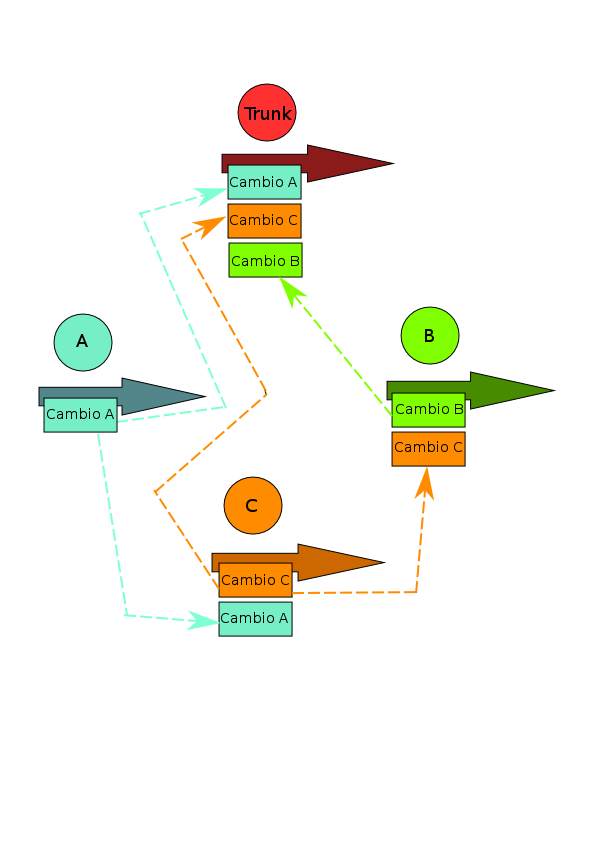
\includegraphics[width=0.5\textwidth]{./imagenes/graficodist.png}
%  \caption{DCVS}
%  \label{fig:01}
%\end{figure}

En el gráfico podemos ver la rama principal (trunk) y varios usuarios (A, B, y C). Cada usuario tiene su propio repositorio con ciertas ramas de
desarrollo, existe una rama principal que lleva las versiones oficiales y sin fallos. Cada usuario guarda su copia local, pero además envía y 
recibe desde y a otros repositorios ciertas ramas de desarrollo y por supuesto la principal que es la que contiene las versiones estables del 
proyecto.

\subsection{Diferentes DCVS}
Entre los más populares encontramos:
\begin{itemize}
\item Git
\item Mercurial
\item Baazar
\item Darcs
\item Monotone
\end{itemize}
Procedemos a explicar Git y Mercurial al ser los más utilizados actualmente. 


\subsection{GIT}
Git es uno de los sistemas de control de versiones distribuidos más usados. Git fue creado por Linus Torvalds y buscaba un sistema que cumpliera
4 requisitos básicos:
\begin{itemize}
\item No se pareciera a CVS
\item Fuera distribuido
\item Seguro frente corrupción, accidental o intencionada
\item Gran rendimiento en las operaciones
\end{itemize} 
Git está escrito en C y en gran parte fue construido para trabajar en el kernel de Linux, lo que quiere decir que desde el primer día ha tenido que mover 
de manera efectiva repositorios de gran tamaño. 

\subsubsection{GIT Es Distribuido}
Cada usuario tiene una copia completa del servidor principal, y cualquiera de ellas podría ser recuperada para reemplazarlo en caso 
de caída o corrupción. Básicamente, no hay un punto de fallo único con git a no ser que haya un punto único. 
\subsubsection{Ramas Locales Sin Coste}
Posiblemente la razón más fuerte a favor de Git que realmente lo hace destacar de casi cualquier otro SCV es su modelo de ramas. Git permite
tener múltiples ramas locales independientes entre sí y se tarda segundos en crear, fusionar, o borrar estas líneas de desarrollo.
Se pueden hacer cosas como: 
\begin{itemize}
\item Crear una rama para probar una idea, volver al punto desde el cual bifurcaste y volver a donde estabas experimentado y fusionarlo. 
\item Tener una rama que siempre contiene sólo lo que va a producción, otra en la que acumulas el trabajo para testear y varias ramas más pequeñas para el trabajo diario.
\item Crear una rama en la que experimentar, darte cuenta de que no va a ninguna parte y borrarla, abandonando todo el trabajo (sin que nadie más lo vea). 
\end{itemize} 
Es importante el que, cuando uno entrega sus cambios a un repositorio remoto, no tienes que subir todas tus ramas: puedes compartir 
sólo una de tus ramas y no todas. De esta forma la gente tiende a sentirse libre para probar nuevas ideas sin preocuparse de tener un 
plan de cómo y cuándo van a mezclar sus cambios o compartirlos con otros.

\subsubsection{GIT Es Local, Rápido y Pequeño}
Al ser local trabaja de forma muy rápida, también te permite trabajar cuando estés sin conexión. Puesde descargar la información del servidor y
trabajar con ella de forma local. Existen pocos comandos que accedan al servidor y los repositorios ocupan muy poco espacio

\subsubsection{EL Área de Montaje}
GIT tiene lo que denomina "área de montaje", o "índice" que es un área intermedia donde puedes configurar el aspecto 
que tendrá tu entrega antes de hacer el commit. Esto también te permite preparar sólo fragmentos de archivos que han sido modificados. Por ejemplo, montas para entregar sólo los cambios 
al principio de un archivo que has estado modificando pero no los cambios del final. Por supuesto, GIT también hace que sea fácil ignorar esta 
funcionalidad en caso de que no queramos tanto nivel de control (simplemente se añade '-a' al commando 'commit'). 

\subsubsection{Diferentes Flujos de Trabajo}
Se puede implementar fácilmente prácitcamente cualquier flujo de trabajo que se nos ocurra.
\begin{itemize}
\item \textbf{Estilo SVN}\\
Forma de trabajo muy común entre aquellos que se pasan de un sistema no distribuido es un flujo de trabajo centralizado. 
Git no permite hacer subir los cambios al servidor si alguien lo ha hecho desde la última vez que nos bajamos los últimos cambios, 
de forma que un modelo centralizado donde todos los desarrolladores entregan al mismo servidor.
\item \textbf{Estilo Responsable Integración}\\
Existe un Responsable de Integración, una persona que entrega al repositorio final, y después un número de desarrolladores se copian 
ese repositorio y hacen sus cambios, luego piden al integrador que integre sus cambios.
\item \textbf{Estilo Dictador y Tenientes}\\
Similar a como lo hacen en el kernel de Linux, donde hay gente que está a cargo de un subsistema específico del proyecto (los tenientes)
e integran todos los cambios que tienen que ver con ese subsistema. Después otro integrador (el dictador) puede recoger los cambios
únicamente de sus tenientes y subirlos al repositorio principal, el cual todo el mundo vuelve a clonar. 
\end{itemize} 

\subsubsection{Uso De GIT}
Se rige por un comportamiento básico de “update-modify-commit”. A continuación se incluye una lista de las instrucciones más comunes 
con su equivalente en SVN:


\textbf{git clone <repositorio> $\rightarrow$} svn checkout <repositorio>\\
\textbf{git init (desde el directorio)  $\rightarrow$}    svn admin create <repositorio>\\
\textbf{git add <fichero>  $\rightarrow$ }  svn add <fichero>\\
\textbf{git rm <fichero>  $\rightarrow$  }  svn rm <fichero>\\
\textbf{git checkout <ruta> $\rightarrow$ }  svn revert <ruta>\\
\textbf{git pull  $\rightarrow$}    svn update\\
\textbf{git commit -a  $\rightarrow$ }   svn commit\\
\textbf{git diff  $\rightarrow$  }  svn diff | less\\
\textbf{git status  $\rightarrow$ }  svn status\\
\textbf{git tag/git branch  $\rightarrow$ }  svn copy <origen> <destino>\\

\subsubsection{Primeros Pasos}
Supongamos que tenemos GIT instalado y un repositorio al algún sitio remoto. 
Una vez hecho esto, tendremos que hacer un checkout cuyo equivalente a esto en git es clone. Vamos a usar el repositorio público de proyectos 
para este ejemplo.\\
En primer lugar se muestran lso pasos para crear un nuevo repositorio en GibHub: Para ello nos damos de alta en GibHub y creamos un nuevo 
repositorio en la web. Los siguientes pasos son para crear un nuevo repositorio local y hacer nuestro primer commit(local) y push(remoto):
\begin{enumerate}
\item mkdir Trabajo-ASO
\item cd Trabajo-ASO
\item git init
\item git add .
\item git commit -a -m 'Primer commit'
\item git remote add origin git@github.com:solidge0/Trabajo-ASO.git
\item git push origin master
\end{enumerate}
Ahora ya tenemos un nuevo repositorio, pero ¿y si este existia y queremos bajarlo?. Fácil:\\


\subsection{Mercurial}

\backmatter % Apéndices, bibliografia ...

% usado en Cliente
\nocite{website:es.wikipedia.org}
\nocite{pdf:Subversion}
\nocite{pdf:Git}

\clearpage
\addcontentsline{toc}{chapter}{Bibliografia y referencias}
\bibliographystyle{plain}
\bibliography{bibliografia}

% This is set up to run with pdflatex.
%---------The file header---------------------------------------------
%---------------------------------------------------------------------
\chapter*{\rlap{GNU Free Documentation License}}
\phantomsection  % so hyperref creates bookmarks
\addcontentsline{toc}{chapter}{GNU Free Documentation License}
%\label{label_fdl}

 \begin{center}

       Version 1.3, 3 November 2008


 Copyright \copyright{} 2000, 2001, 2002, 2007, 2008  Free Software Foundation, Inc.
 
 \bigskip
 
     <http://fsf.org/>
  
 \bigskip
 
 Everyone is permitted to copy and distribute verbatim copies
 of this license document, but changing it is not allowed.
\end{center}


\begin{center}
{\bf\large Preamble}
\end{center}

The purpose of this License is to make a manual, textbook, or other
functional and useful document ``free'' in the sense of freedom: to
assure everyone the effective freedom to copy and redistribute it,
with or without modifying it, either commercially or noncommercially.
Secondarily, this License preserves for the author and publisher a way
to get credit for their work, while not being considered responsible
for modifications made by others.

This License is a kind of ``copyleft'', which means that derivative
works of the document must themselves be free in the same sense.  It
complements the GNU General Public License, which is a copyleft
license designed for free software.

We have designed this License in order to use it for manuals for free
software, because free software needs free documentation: a free
program should come with manuals providing the same freedoms that the
software does.  But this License is not limited to software manuals;
it can be used for any textual work, regardless of subject matter or
whether it is published as a printed book.  We recommend this License
principally for works whose purpose is instruction or reference.


\begin{center}
{\Large\bf 1. APPLICABILITY AND DEFINITIONS\par}
\phantomsection
\addcontentsline{toc}{section}{1. APPLICABILITY AND DEFINITIONS}
\end{center}

This License applies to any manual or other work, in any medium, that
contains a notice placed by the copyright holder saying it can be
distributed under the terms of this License.  Such a notice grants a
world-wide, royalty-free license, unlimited in duration, to use that
work under the conditions stated herein.  The ``\textbf{Document}'', below,
refers to any such manual or work.  Any member of the public is a
licensee, and is addressed as ``\textbf{you}''.  You accept the license if you
copy, modify or distribute the work in a way requiring permission
under copyright law.

A ``\textbf{Modified Version}'' of the Document means any work containing the
Document or a portion of it, either copied verbatim, or with
modifications and/or translated into another language.

A ``\textbf{Secondary Section}'' is a named appendix or a front-matter section of
the Document that deals exclusively with the relationship of the
publishers or authors of the Document to the Document's overall subject
(or to related matters) and contains nothing that could fall directly
within that overall subject.  (Thus, if the Document is in part a
textbook of mathematics, a Secondary Section may not explain any
mathematics.)  The relationship could be a matter of historical
connection with the subject or with related matters, or of legal,
commercial, philosophical, ethical or political position regarding
them.

The ``\textbf{Invariant Sections}'' are certain Secondary Sections whose titles
are designated, as being those of Invariant Sections, in the notice
that says that the Document is released under this License.  If a
section does not fit the above definition of Secondary then it is not
allowed to be designated as Invariant.  The Document may contain zero
Invariant Sections.  If the Document does not identify any Invariant
Sections then there are none.

The ``\textbf{Cover Texts}'' are certain short passages of text that are listed,
as Front-Cover Texts or Back-Cover Texts, in the notice that says that
the Document is released under this License.  A Front-Cover Text may
be at most 5 words, and a Back-Cover Text may be at most 25 words.

A ``\textbf{Transparent}'' copy of the Document means a machine-readable copy,
represented in a format whose specification is available to the
general public, that is suitable for revising the document
straightforwardly with generic text editors or (for images composed of
pixels) generic paint programs or (for drawings) some widely available
drawing editor, and that is suitable for input to text formatters or
for automatic translation to a variety of formats suitable for input
to text formatters.  A copy made in an otherwise Transparent file
format whose markup, or absence of markup, has been arranged to thwart
or discourage subsequent modification by readers is not Transparent.
An image format is not Transparent if used for any substantial amount
of text.  A copy that is not ``Transparent'' is called ``\textbf{Opaque}''.

Examples of suitable formats for Transparent copies include plain
ASCII without markup, Texinfo input format, LaTeX input format, SGML
or XML using a publicly available DTD, and standard-conforming simple
HTML, PostScript or PDF designed for human modification.  Examples of
transparent image formats include PNG, XCF and JPG.  Opaque formats
include proprietary formats that can be read and edited only by
proprietary word processors, SGML or XML for which the DTD and/or
processing tools are not generally available, and the
machine-generated HTML, PostScript or PDF produced by some word
processors for output purposes only.

The ``\textbf{Title Page}'' means, for a printed book, the title page itself,
plus such following pages as are needed to hold, legibly, the material
this License requires to appear in the title page.  For works in
formats which do not have any title page as such, ``Title Page'' means
the text near the most prominent appearance of the work's title,
preceding the beginning of the body of the text.

The ``\textbf{publisher}'' means any person or entity that distributes
copies of the Document to the public.

A section ``\textbf{Entitled XYZ}'' means a named subunit of the Document whose
title either is precisely XYZ or contains XYZ in parentheses following
text that translates XYZ in another language.  (Here XYZ stands for a
specific section name mentioned below, such as ``\textbf{Acknowledgements}'',
``\textbf{Dedications}'', ``\textbf{Endorsements}'', or ``\textbf{History}''.)  
To ``\textbf{Preserve the Title}''
of such a section when you modify the Document means that it remains a
section ``Entitled XYZ'' according to this definition.

The Document may include Warranty Disclaimers next to the notice which
states that this License applies to the Document.  These Warranty
Disclaimers are considered to be included by reference in this
License, but only as regards disclaiming warranties: any other
implication that these Warranty Disclaimers may have is void and has
no effect on the meaning of this License.


\begin{center}
{\Large\bf 2. VERBATIM COPYING\par}
\phantomsection
\addcontentsline{toc}{section}{2. VERBATIM COPYING}
\end{center}

You may copy and distribute the Document in any medium, either
commercially or noncommercially, provided that this License, the
copyright notices, and the license notice saying this License applies
to the Document are reproduced in all copies, and that you add no other
conditions whatsoever to those of this License.  You may not use
technical measures to obstruct or control the reading or further
copying of the copies you make or distribute.  However, you may accept
compensation in exchange for copies.  If you distribute a large enough
number of copies you must also follow the conditions in section~3.

You may also lend copies, under the same conditions stated above, and
you may publicly display copies.


\begin{center}
{\Large\bf 3. COPYING IN QUANTITY\par}
\phantomsection
\addcontentsline{toc}{section}{3. COPYING IN QUANTITY}
\end{center}


If you publish printed copies (or copies in media that commonly have
printed covers) of the Document, numbering more than 100, and the
Document's license notice requires Cover Texts, you must enclose the
copies in covers that carry, clearly and legibly, all these Cover
Texts: Front-Cover Texts on the front cover, and Back-Cover Texts on
the back cover.  Both covers must also clearly and legibly identify
you as the publisher of these copies.  The front cover must present
the full title with all words of the title equally prominent and
visible.  You may add other material on the covers in addition.
Copying with changes limited to the covers, as long as they preserve
the title of the Document and satisfy these conditions, can be treated
as verbatim copying in other respects.

If the required texts for either cover are too voluminous to fit
legibly, you should put the first ones listed (as many as fit
reasonably) on the actual cover, and continue the rest onto adjacent
pages.

If you publish or distribute Opaque copies of the Document numbering
more than 100, you must either include a machine-readable Transparent
copy along with each Opaque copy, or state in or with each Opaque copy
a computer-network location from which the general network-using
public has access to download using public-standard network protocols
a complete Transparent copy of the Document, free of added material.
If you use the latter option, you must take reasonably prudent steps,
when you begin distribution of Opaque copies in quantity, to ensure
that this Transparent copy will remain thus accessible at the stated
location until at least one year after the last time you distribute an
Opaque copy (directly or through your agents or retailers) of that
edition to the public.

It is requested, but not required, that you contact the authors of the
Document well before redistributing any large number of copies, to give
them a chance to provide you with an updated version of the Document.


\begin{center}
{\Large\bf 4. MODIFICATIONS\par}
\phantomsection
\addcontentsline{toc}{section}{4. MODIFICATIONS}
\end{center}

You may copy and distribute a Modified Version of the Document under
the conditions of sections 2 and 3 above, provided that you release
the Modified Version under precisely this License, with the Modified
Version filling the role of the Document, thus licensing distribution
and modification of the Modified Version to whoever possesses a copy
of it.  In addition, you must do these things in the Modified Version:

\begin{itemize}
\item[A.] 
   Use in the Title Page (and on the covers, if any) a title distinct
   from that of the Document, and from those of previous versions
   (which should, if there were any, be listed in the History section
   of the Document).  You may use the same title as a previous version
   if the original publisher of that version gives permission.
   
\item[B.]
   List on the Title Page, as authors, one or more persons or entities
   responsible for authorship of the modifications in the Modified
   Version, together with at least five of the principal authors of the
   Document (all of its principal authors, if it has fewer than five),
   unless they release you from this requirement.
   
\item[C.]
   State on the Title page the name of the publisher of the
   Modified Version, as the publisher.
   
\item[D.]
   Preserve all the copyright notices of the Document.
   
\item[E.]
   Add an appropriate copyright notice for your modifications
   adjacent to the other copyright notices.
   
\item[F.]
   Include, immediately after the copyright notices, a license notice
   giving the public permission to use the Modified Version under the
   terms of this License, in the form shown in the Addendum below.
   
\item[G.]
   Preserve in that license notice the full lists of Invariant Sections
   and required Cover Texts given in the Document's license notice.
   
\item[H.]
   Include an unaltered copy of this License.
   
\item[I.]
   Preserve the section Entitled ``History'', Preserve its Title, and add
   to it an item stating at least the title, year, new authors, and
   publisher of the Modified Version as given on the Title Page.  If
   there is no section Entitled ``History'' in the Document, create one
   stating the title, year, authors, and publisher of the Document as
   given on its Title Page, then add an item describing the Modified
   Version as stated in the previous sentence.
   
\item[J.]
   Preserve the network location, if any, given in the Document for
   public access to a Transparent copy of the Document, and likewise
   the network locations given in the Document for previous versions
   it was based on.  These may be placed in the ``History'' section.
   You may omit a network location for a work that was published at
   least four years before the Document itself, or if the original
   publisher of the version it refers to gives permission.
   
\item[K.]
   For any section Entitled ``Acknowledgements'' or ``Dedications'',
   Preserve the Title of the section, and preserve in the section all
   the substance and tone of each of the contributor acknowledgements
   and/or dedications given therein.
   
\item[L.]
   Preserve all the Invariant Sections of the Document,
   unaltered in their text and in their titles.  Section numbers
   or the equivalent are not considered part of the section titles.
   
\item[M.]
   Delete any section Entitled ``Endorsements''.  Such a section
   may not be included in the Modified Version.
   
\item[N.]
   Do not retitle any existing section to be Entitled ``Endorsements''
   or to conflict in title with any Invariant Section.
   
\item[O.]
   Preserve any Warranty Disclaimers.
\end{itemize}

If the Modified Version includes new front-matter sections or
appendices that qualify as Secondary Sections and contain no material
copied from the Document, you may at your option designate some or all
of these sections as invariant.  To do this, add their titles to the
list of Invariant Sections in the Modified Version's license notice.
These titles must be distinct from any other section titles.

You may add a section Entitled ``Endorsements'', provided it contains
nothing but endorsements of your Modified Version by various
parties---for example, statements of peer review or that the text has
been approved by an organization as the authoritative definition of a
standard.

You may add a passage of up to five words as a Front-Cover Text, and a
passage of up to 25 words as a Back-Cover Text, to the end of the list
of Cover Texts in the Modified Version.  Only one passage of
Front-Cover Text and one of Back-Cover Text may be added by (or
through arrangements made by) any one entity.  If the Document already
includes a cover text for the same cover, previously added by you or
by arrangement made by the same entity you are acting on behalf of,
you may not add another; but you may replace the old one, on explicit
permission from the previous publisher that added the old one.

The author(s) and publisher(s) of the Document do not by this License
give permission to use their names for publicity for or to assert or
imply endorsement of any Modified Version.


\begin{center}
{\Large\bf 5. COMBINING DOCUMENTS\par}
\phantomsection
\addcontentsline{toc}{section}{5. COMBINING DOCUMENTS}
\end{center}


You may combine the Document with other documents released under this
License, under the terms defined in section~4 above for modified
versions, provided that you include in the combination all of the
Invariant Sections of all of the original documents, unmodified, and
list them all as Invariant Sections of your combined work in its
license notice, and that you preserve all their Warranty Disclaimers.

The combined work need only contain one copy of this License, and
multiple identical Invariant Sections may be replaced with a single
copy.  If there are multiple Invariant Sections with the same name but
different contents, make the title of each such section unique by
adding at the end of it, in parentheses, the name of the original
author or publisher of that section if known, or else a unique number.
Make the same adjustment to the section titles in the list of
Invariant Sections in the license notice of the combined work.

In the combination, you must combine any sections Entitled ``History''
in the various original documents, forming one section Entitled
``History''; likewise combine any sections Entitled ``Acknowledgements'',
and any sections Entitled ``Dedications''.  You must delete all sections
Entitled ``Endorsements''.

\begin{center}
{\Large\bf 6. COLLECTIONS OF DOCUMENTS\par}
\phantomsection
\addcontentsline{toc}{section}{6. COLLECTIONS OF DOCUMENTS}
\end{center}

You may make a collection consisting of the Document and other documents
released under this License, and replace the individual copies of this
License in the various documents with a single copy that is included in
the collection, provided that you follow the rules of this License for
verbatim copying of each of the documents in all other respects.

You may extract a single document from such a collection, and distribute
it individually under this License, provided you insert a copy of this
License into the extracted document, and follow this License in all
other respects regarding verbatim copying of that document.


\begin{center}
{\Large\bf 7. AGGREGATION WITH INDEPENDENT WORKS\par}
\phantomsection
\addcontentsline{toc}{section}{7. AGGREGATION WITH INDEPENDENT WORKS}
\end{center}


A compilation of the Document or its derivatives with other separate
and independent documents or works, in or on a volume of a storage or
distribution medium, is called an ``aggregate'' if the copyright
resulting from the compilation is not used to limit the legal rights
of the compilation's users beyond what the individual works permit.
When the Document is included in an aggregate, this License does not
apply to the other works in the aggregate which are not themselves
derivative works of the Document.

If the Cover Text requirement of section~3 is applicable to these
copies of the Document, then if the Document is less than one half of
the entire aggregate, the Document's Cover Texts may be placed on
covers that bracket the Document within the aggregate, or the
electronic equivalent of covers if the Document is in electronic form.
Otherwise they must appear on printed covers that bracket the whole
aggregate.


\begin{center}
{\Large\bf 8. TRANSLATION\par}
\phantomsection
\addcontentsline{toc}{section}{8. TRANSLATION}
\end{center}


Translation is considered a kind of modification, so you may
distribute translations of the Document under the terms of section~4.
Replacing Invariant Sections with translations requires special
permission from their copyright holders, but you may include
translations of some or all Invariant Sections in addition to the
original versions of these Invariant Sections.  You may include a
translation of this License, and all the license notices in the
Document, and any Warranty Disclaimers, provided that you also include
the original English version of this License and the original versions
of those notices and disclaimers.  In case of a disagreement between
the translation and the original version of this License or a notice
or disclaimer, the original version will prevail.

If a section in the Document is Entitled ``Acknowledgements'',
``Dedications'', or ``History'', the requirement (section~4) to Preserve
its Title (section~1) will typically require changing the actual
title.


\begin{center}
{\Large\bf 9. TERMINATION\par}
\phantomsection
\addcontentsline{toc}{section}{9. TERMINATION}
\end{center}


You may not copy, modify, sublicense, or distribute the Document
except as expressly provided under this License.  Any attempt
otherwise to copy, modify, sublicense, or distribute it is void, and
will automatically terminate your rights under this License.

However, if you cease all violation of this License, then your license
from a particular copyright holder is reinstated (a) provisionally,
unless and until the copyright holder explicitly and finally
terminates your license, and (b) permanently, if the copyright holder
fails to notify you of the violation by some reasonable means prior to
60 days after the cessation.

Moreover, your license from a particular copyright holder is
reinstated permanently if the copyright holder notifies you of the
violation by some reasonable means, this is the first time you have
received notice of violation of this License (for any work) from that
copyright holder, and you cure the violation prior to 30 days after
your receipt of the notice.

Termination of your rights under this section does not terminate the
licenses of parties who have received copies or rights from you under
this License.  If your rights have been terminated and not permanently
reinstated, receipt of a copy of some or all of the same material does
not give you any rights to use it.


\begin{center}
{\Large\bf 10. FUTURE REVISIONS OF THIS LICENSE\par}
\phantomsection
\addcontentsline{toc}{section}{10. FUTURE REVISIONS OF THIS LICENSE}
\end{center}


The Free Software Foundation may publish new, revised versions
of the GNU Free Documentation License from time to time.  Such new
versions will be similar in spirit to the present version, but may
differ in detail to address new problems or concerns.  See
http://www.gnu.org/copyleft/.

Each version of the License is given a distinguishing version number.
If the Document specifies that a particular numbered version of this
License ``or any later version'' applies to it, you have the option of
following the terms and conditions either of that specified version or
of any later version that has been published (not as a draft) by the
Free Software Foundation.  If the Document does not specify a version
number of this License, you may choose any version ever published (not
as a draft) by the Free Software Foundation.  If the Document
specifies that a proxy can decide which future versions of this
License can be used, that proxy's public statement of acceptance of a
version permanently authorizes you to choose that version for the
Document.


\begin{center}
{\Large\bf 11. RELICENSING\par}
\phantomsection
\addcontentsline{toc}{section}{11. RELICENSING}
\end{center}


``Massive Multiauthor Collaboration Site'' (or ``MMC Site'') means any
World Wide Web server that publishes copyrightable works and also
provides prominent facilities for anybody to edit those works.  A
public wiki that anybody can edit is an example of such a server.  A
``Massive Multiauthor Collaboration'' (or ``MMC'') contained in the
site means any set of copyrightable works thus published on the MMC
site.

``CC-BY-SA'' means the Creative Commons Attribution-Share Alike 3.0
license published by Creative Commons Corporation, a not-for-profit
corporation with a principal place of business in San Francisco,
California, as well as future copyleft versions of that license
published by that same organization.

``Incorporate'' means to publish or republish a Document, in whole or
in part, as part of another Document.

An MMC is ``eligible for relicensing'' if it is licensed under this
License, and if all works that were first published under this License
somewhere other than this MMC, and subsequently incorporated in whole
or in part into the MMC, (1) had no cover texts or invariant sections,
and (2) were thus incorporated prior to November 1, 2008.

The operator of an MMC Site may republish an MMC contained in the site
under CC-BY-SA on the same site at any time before August 1, 2009,
provided the MMC is eligible for relicensing.


\begin{center}
{\Large\bf ADDENDUM: How to use this License for your documents\par}
\phantomsection
\addcontentsline{toc}{section}{ADDENDUM: How to use this License for your documents}
\end{center}

To use this License in a document you have written, include a copy of
the License in the document and put the following copyright and
license notices just after the title page:

\bigskip
\begin{quote}
    Copyright \copyright{}  YEAR  YOUR NAME.
    Permission is granted to copy, distribute and/or modify this document
    under the terms of the GNU Free Documentation License, Version 1.3
    or any later version published by the Free Software Foundation;
    with no Invariant Sections, no Front-Cover Texts, and no Back-Cover Texts.
    A copy of the license is included in the section entitled ``GNU
    Free Documentation License''.
\end{quote}
\bigskip
    
If you have Invariant Sections, Front-Cover Texts and Back-Cover Texts,
replace the ``with \dots\ Texts.'' line with this:

\bigskip
\begin{quote}
    with the Invariant Sections being LIST THEIR TITLES, with the
    Front-Cover Texts being LIST, and with the Back-Cover Texts being LIST.
\end{quote}
\bigskip
    
If you have Invariant Sections without Cover Texts, or some other
combination of the three, merge those two alternatives to suit the
situation.

If your document contains nontrivial examples of program code, we
recommend releasing these examples in parallel under your choice of
free software license, such as the GNU General Public License,
to permit their use in free software.

%---------------------------------------------------------------------


\end{document}
